% Options for packages loaded elsewhere
\PassOptionsToPackage{unicode}{hyperref}
\PassOptionsToPackage{hyphens}{url}
%
\documentclass[
]{article}
\usepackage{amsmath,amssymb}
\usepackage{iftex}
\ifPDFTeX
  \usepackage[T1]{fontenc}
  \usepackage[utf8]{inputenc}
  \usepackage{textcomp} % provide euro and other symbols
\else % if luatex or xetex
  \usepackage{unicode-math} % this also loads fontspec
  \defaultfontfeatures{Scale=MatchLowercase}
  \defaultfontfeatures[\rmfamily]{Ligatures=TeX,Scale=1}
\fi
\usepackage{lmodern}
\ifPDFTeX\else
  % xetex/luatex font selection
\fi
% Use upquote if available, for straight quotes in verbatim environments
\IfFileExists{upquote.sty}{\usepackage{upquote}}{}
\IfFileExists{microtype.sty}{% use microtype if available
  \usepackage[]{microtype}
  \UseMicrotypeSet[protrusion]{basicmath} % disable protrusion for tt fonts
}{}
\makeatletter
\@ifundefined{KOMAClassName}{% if non-KOMA class
  \IfFileExists{parskip.sty}{%
    \usepackage{parskip}
  }{% else
    \setlength{\parindent}{0pt}
    \setlength{\parskip}{6pt plus 2pt minus 1pt}}
}{% if KOMA class
  \KOMAoptions{parskip=half}}
\makeatother
\usepackage{xcolor}
\usepackage[margin=1in]{geometry}
\usepackage{longtable,booktabs,array}
\usepackage{calc} % for calculating minipage widths
% Correct order of tables after \paragraph or \subparagraph
\usepackage{etoolbox}
\makeatletter
\patchcmd\longtable{\par}{\if@noskipsec\mbox{}\fi\par}{}{}
\makeatother
% Allow footnotes in longtable head/foot
\IfFileExists{footnotehyper.sty}{\usepackage{footnotehyper}}{\usepackage{footnote}}
\makesavenoteenv{longtable}
\usepackage{graphicx}
\makeatletter
\def\maxwidth{\ifdim\Gin@nat@width>\linewidth\linewidth\else\Gin@nat@width\fi}
\def\maxheight{\ifdim\Gin@nat@height>\textheight\textheight\else\Gin@nat@height\fi}
\makeatother
% Scale images if necessary, so that they will not overflow the page
% margins by default, and it is still possible to overwrite the defaults
% using explicit options in \includegraphics[width, height, ...]{}
\setkeys{Gin}{width=\maxwidth,height=\maxheight,keepaspectratio}
% Set default figure placement to htbp
\makeatletter
\def\fps@figure{htbp}
\makeatother
\setlength{\emergencystretch}{3em} % prevent overfull lines
\providecommand{\tightlist}{%
  \setlength{\itemsep}{0pt}\setlength{\parskip}{0pt}}
\setcounter{secnumdepth}{5}
\newlength{\cslhangindent}
\setlength{\cslhangindent}{1.5em}
\newlength{\csllabelwidth}
\setlength{\csllabelwidth}{3em}
\newlength{\cslentryspacingunit} % times entry-spacing
\setlength{\cslentryspacingunit}{\parskip}
\newenvironment{CSLReferences}[2] % #1 hanging-ident, #2 entry spacing
 {% don't indent paragraphs
  \setlength{\parindent}{0pt}
  % turn on hanging indent if param 1 is 1
  \ifodd #1
  \let\oldpar\par
  \def\par{\hangindent=\cslhangindent\oldpar}
  \fi
  % set entry spacing
  \setlength{\parskip}{#2\cslentryspacingunit}
 }%
 {}
\usepackage{calc}
\newcommand{\CSLBlock}[1]{#1\hfill\break}
\newcommand{\CSLLeftMargin}[1]{\parbox[t]{\csllabelwidth}{#1}}
\newcommand{\CSLRightInline}[1]{\parbox[t]{\linewidth - \csllabelwidth}{#1}\break}
\newcommand{\CSLIndent}[1]{\hspace{\cslhangindent}#1}
\ifLuaTeX
  \usepackage{selnolig}  % disable illegal ligatures
\fi
\IfFileExists{bookmark.sty}{\usepackage{bookmark}}{\usepackage{hyperref}}
\IfFileExists{xurl.sty}{\usepackage{xurl}}{} % add URL line breaks if available
\urlstyle{same}
\hypersetup{
  pdftitle={Lessons learned: creating tutorials teaching Agent-Based Modelling for Archaeologists},
  hidelinks,
  pdfcreator={LaTeX via pandoc}}

\title{Lessons learned: creating tutorials teaching Agent-Based Modelling for Archaeologists}
\author{true \and true \and true \and true \and true \and true \and true \and true \and true}
\date{29 February 2024}

\begin{document}
\maketitle

{
\setcounter{tocdepth}{2}
\tableofcontents
}
\hypertarget{introduction}{%
\section{Introduction}\label{introduction}}

ABM application increased in Archaeology

No formal training

EU project

\hypertarget{method}{%
\section{Method}\label{method}}

During the project we have developed tutorials. The tutorials were first designed using storyboards which were later converted into tutorials using NetLOGO Web (\url{https://www.netlogoweb.org/launch}) and Javascript (). The tutorials were developed together and we worked together using GitHub (\url{https://github.com/lljvdk/EU-ABMA/}). During the project initial testing was done with all authors and issues in GitHub were used to tackle bugs.

The tutorial were tested during various online and in-person conferences. In addition, we also had students working with the tutorials at Saxion Universty of applied sciences and Leiden University. We used the feedback of the participants to improve the tutorials. The feedback was obtained structurally using two surveys using Qualtrics. The participants of the events were asked to answer questions of a survey before participating. We used the answers to understand what the background of the participants was and to get an estimate of their level of knowledge in relation to ABM (see appendix \ldots{} for the questions). After the participants worked with the tutorials during the event they were asked to answer a second survey. Questions of this survey were aimed at the measuring the effectiveness of the tutorials and getting feedback on the workshop and tutorials (see appendix \ldots{} for the questions). For some events participants had to register beforehand and we were able to send the pre-workshop survey by email. At other events no registration was possible or necessary and the pre-workshop survey was given at the start of the event. The post-workshop survey was distributed using QR-codes or links at the end of the workshop during the event. After each event we have improved the tutorials based on the received feedback.

\begin{longtable}[]{@{}
  >{\raggedright\arraybackslash}p{(\columnwidth - 8\tabcolsep) * \real{0.2000}}
  >{\raggedright\arraybackslash}p{(\columnwidth - 8\tabcolsep) * \real{0.2000}}
  >{\raggedright\arraybackslash}p{(\columnwidth - 8\tabcolsep) * \real{0.2000}}
  >{\raggedright\arraybackslash}p{(\columnwidth - 8\tabcolsep) * \real{0.2000}}
  >{\raggedright\arraybackslash}p{(\columnwidth - 8\tabcolsep) * \real{0.2000}}@{}}
\caption{Conferences, events and situations were the workshops given and the tutorials were tested.}\tabularnewline
\toprule\noalign{}
\begin{minipage}[b]{\linewidth}\raggedright
Conference or event
\end{minipage} & \begin{minipage}[b]{\linewidth}\raggedright
Period
\end{minipage} & \begin{minipage}[b]{\linewidth}\raggedright
Online, in person or hybrid
\end{minipage} & \begin{minipage}[b]{\linewidth}\raggedright
Number of participants
\end{minipage} & \begin{minipage}[b]{\linewidth}\raggedright
Number of registrations
\end{minipage} \\
\midrule\noalign{}
\endfirsthead
\toprule\noalign{}
\begin{minipage}[b]{\linewidth}\raggedright
Conference or event
\end{minipage} & \begin{minipage}[b]{\linewidth}\raggedright
Period
\end{minipage} & \begin{minipage}[b]{\linewidth}\raggedright
Online, in person or hybrid
\end{minipage} & \begin{minipage}[b]{\linewidth}\raggedright
Number of participants
\end{minipage} & \begin{minipage}[b]{\linewidth}\raggedright
Number of registrations
\end{minipage} \\
\midrule\noalign{}
\endhead
\bottomrule\noalign{}
\endlastfoot
CAA Amsterdam & April 2023 & In person & & \\
EAA Belfast & August 2023 & In person & & No registration \\
CAA-DE/NL-Fl Online workshop & October 2023 & Online & & \\
Reuvensdagen & November 2023 & In person & & No registration \\
CAA-UK & November 2023 & Hybrid & & \\
Leiden (course) & December 2023 & In person & & \\
Aarhus & January/February 2024 & Online & 176 & \textgreater500 \\
Saxion & March 2023-January 2024 & In person & 18 & \\
\end{longtable}

The surveys were analysed using R (R Core Team 2023). The following packages were used for analyses: ggplot2 (Wickham 2016), dplyr (Wickham et al. 2023), tidyr (Wickham, Vaughan and Girlich 2023), forcats(Wickham 2023a), lubridate (Grolemund and Wickham 2011) and stringr (Wickham 2023b). The date and the code is available at \url{https://github.com/RonaldVisser/ABM_tutorials} and (\ldots{} insert Zenodo reference\ldots)

\hypertarget{results}{%
\section{Results}\label{results}}

\hypertarget{tutorials}{%
\subsection{Tutorials}\label{tutorials}}

\hypertarget{before-tutorial}{%
\subsection{Before tutorial}\label{before-tutorial}}

A large proportion of the participants of the workshops gave us information using the survey before the workshops 172 of (\ldots total number\ldots) participants. The respondents came from many different countries all over the world (see Figure \ref{fig:nationality}. The number of female respondents slightly outnumber the male ones and a small group did not share their gender and two were non-binary (see Figure \ref{fig:gender-age}). The ages of the respondents ranged from below 20 to over 70, reaching people in different age classes, although the majority was aged between 20 and 40. It seems that the different events also had a slightly different distribution of both gender and age. For example, more older people attended the workshop at the CAA conference in April 2023 and more male people were present during the workshop at the Reuvensdagen in November 2023.

students???

\begin{figure}
\centering
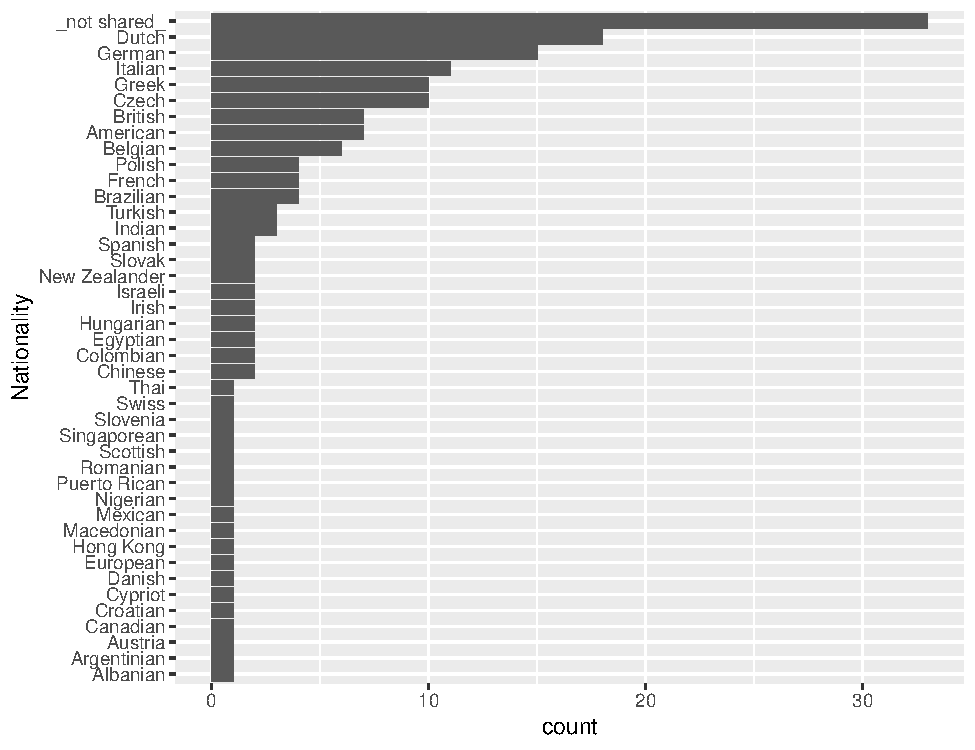
\includegraphics{paper_files/figure-latex/nationality-1.pdf}
\caption{\label{fig:nationality}The nationality of the participants that filled in the survey.}
\end{figure}

\begin{figure}
\centering
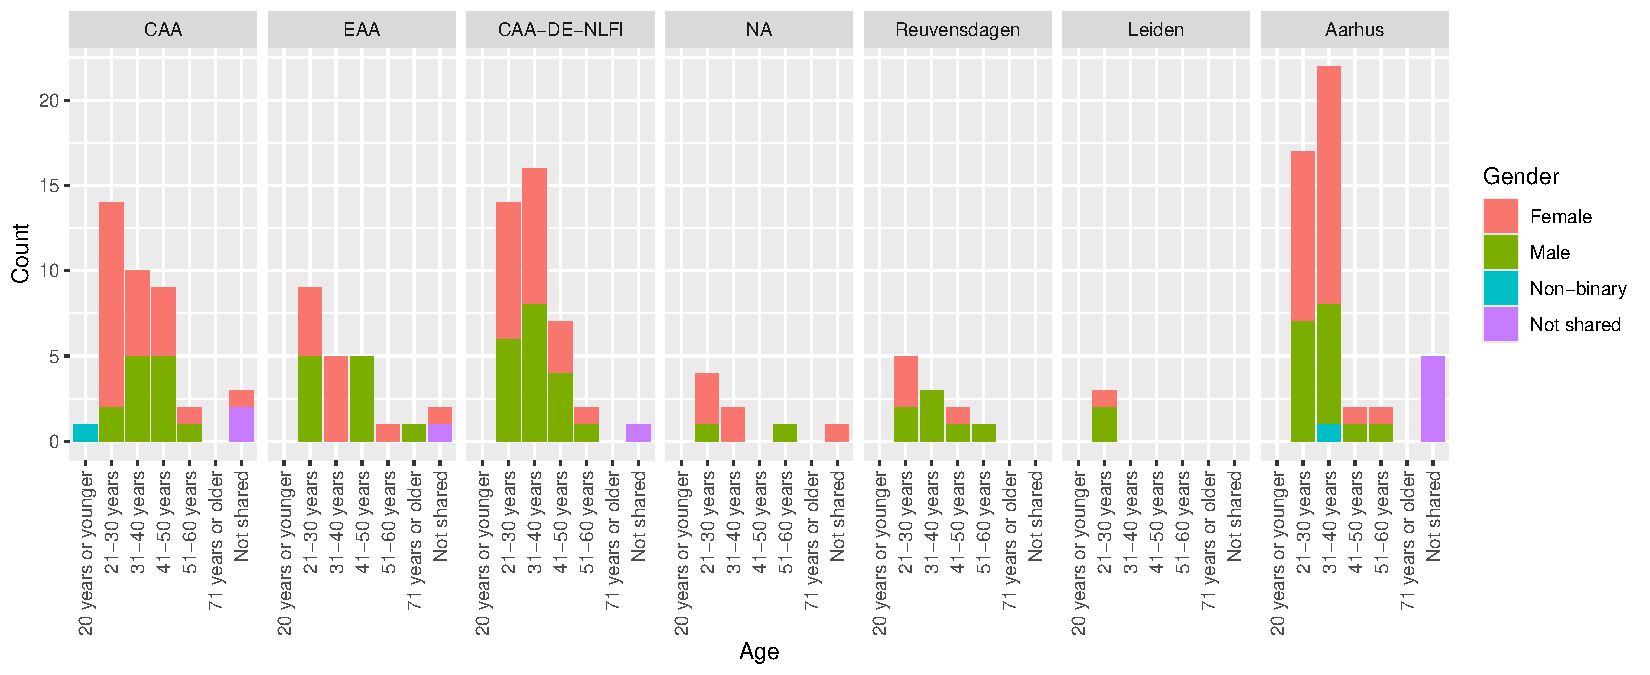
\includegraphics{paper_files/figure-latex/gender-age-1.pdf}
\caption{\label{fig:gender-age}The gender and age of the respondents for each workshop}
\end{figure}

Most of the respondents had several skills with computer applications in archaeology (see Figure \ref{fig:computer-skills}), and many of them did have some knowledge of ABM, although a large group was completely new to the subject. The majority had never applied ABM before participating in the workshops with 14 having applied ABM. It is interesting to note that many respondents did know what kind of software was available for ABM (see Figure \ref{fig:abm-knowledge}).

\begin{figure}
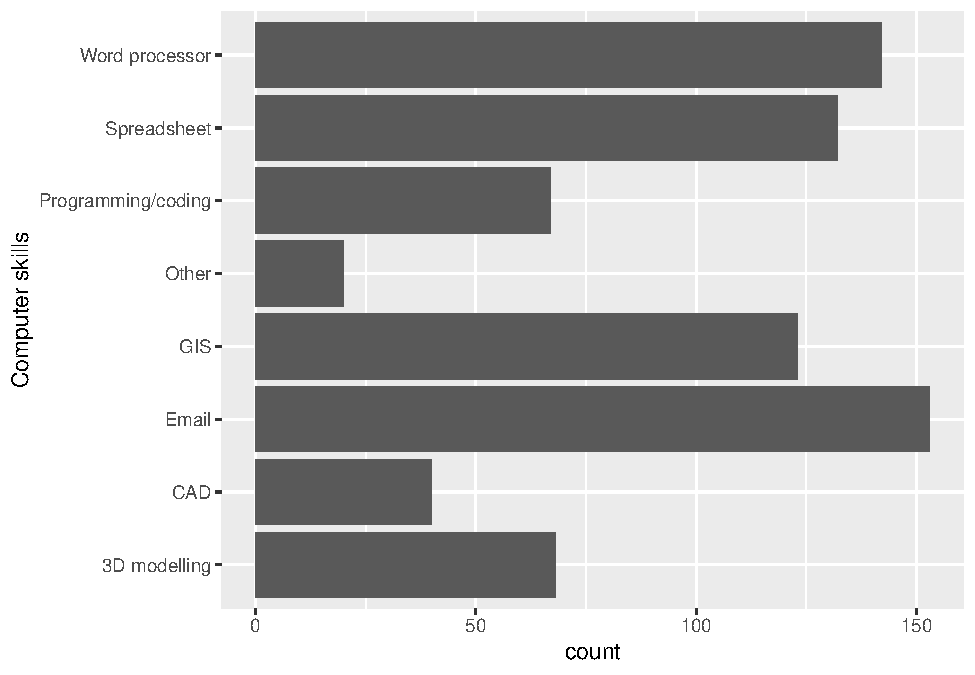
\includegraphics[width=0.5\linewidth]{paper_files/figure-latex/computer-skills-1} \caption{The computer skills of the respondents.}\label{fig:computer-skills}
\end{figure}

\begin{figure}
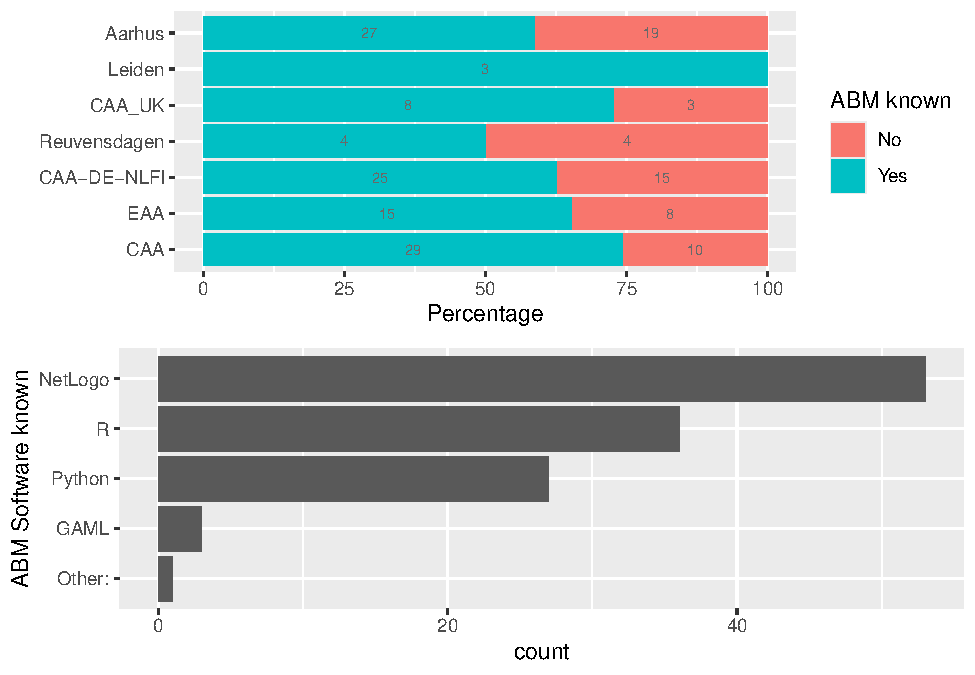
\includegraphics[width=0.5\linewidth]{paper_files/figure-latex/abm-knowledge-1} 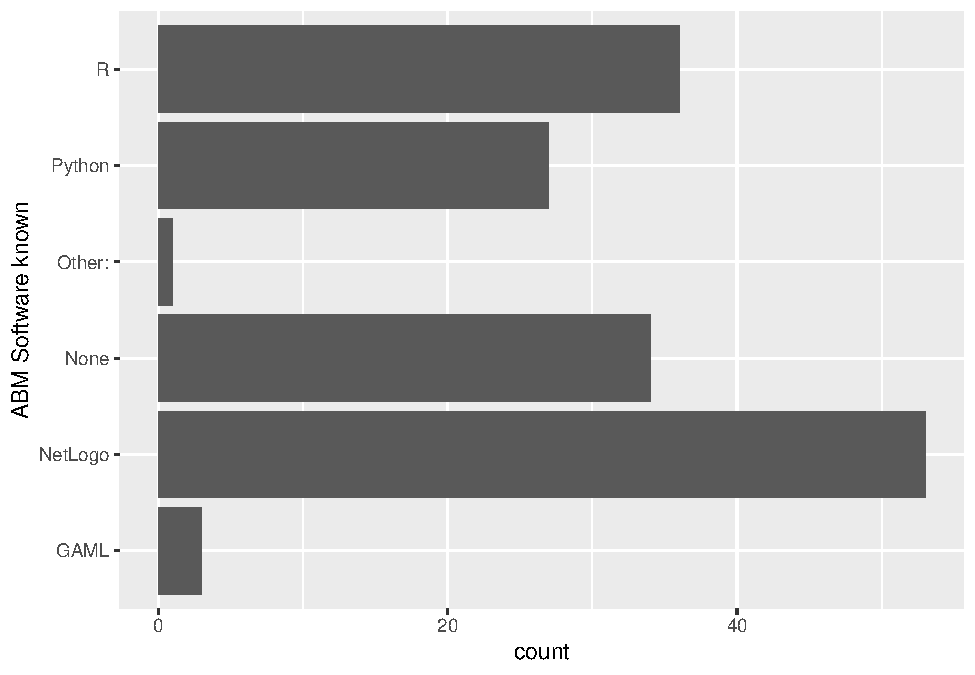
\includegraphics[width=0.5\linewidth]{paper_files/figure-latex/abm-knowledge-2} \caption{Respondents knowledge and experience with ABM.}\label{fig:abm-knowledge}
\end{figure}

\hypertarget{after-tutorial}{%
\subsection{After tutorial}\label{after-tutorial}}

\hypertarget{final-tutorials}{%
\subsection{Final tutorials}\label{final-tutorials}}

\hypertarget{dissemination-of-tutorials}{%
\subsection{Dissemination of tutorials}\label{dissemination-of-tutorials}}

Website

\hypertarget{conclusion}{%
\section{Conclusion}\label{conclusion}}

Lessons learned

Future aspects

\hypertarget{acknowledgements}{%
\section{Acknowledgements}\label{acknowledgements}}

The roles of this paper according to CReDiT (Contributor Roles Taxonomy):

Kenneth Aitchison

Tom Brughmans

Annemarie Jutte

Laura van der Knaap

Karsten Lambers

Doug Rocks-Macqueen (Software)

Iza Romanowska

Ronald M. Visser (Writing -- original draft, Formal Analysis, Visualization)

\hypertarget{references}{%
\section*{References}\label{references}}
\addcontentsline{toc}{section}{References}

\hypertarget{refs}{}
\begin{CSLReferences}{1}{0}
\leavevmode\vadjust pre{\hypertarget{ref-grolemund2011}{}}%
Grolemund, G and Wickham, H. 2011 \href{https://www.jstatsoft.org/v40/i03/}{Dates and times made easy with lubridate}. \emph{Journal of Statistical Software} 40(3): 125.

\leavevmode\vadjust pre{\hypertarget{ref-rcoreteam2023}{}}%
R Core Team. 2023 \emph{\href{https://www.R-project.org/}{R: A language and environment for statistical computing}}.

\leavevmode\vadjust pre{\hypertarget{ref-wickham2016}{}}%
Wickham, H. 2016. \emph{\href{http://ggplot2.org}{ggplot2: Elegant graphics for data analysis}}. Springer-Verlag New York.

\leavevmode\vadjust pre{\hypertarget{ref-wickham2023b}{}}%
Wickham, H. 2023a \emph{\href{https://forcats.tidyverse.org/}{Forcats: Tools for working with categorical variables (factors)}}.

\leavevmode\vadjust pre{\hypertarget{ref-wickham2023c}{}}%
Wickham, H. 2023b \emph{\href{https://stringr.tidyverse.org}{Stringr: Simple, consistent wrappers for common string operations}}.

\leavevmode\vadjust pre{\hypertarget{ref-wickham2023a}{}}%
Wickham, H, François, R, Henry, L, Müller, K and Vaughan, D. 2023 \emph{\href{https://dplyr.tidyverse.org}{Dplyr: A grammar of data manipulation}}.

\leavevmode\vadjust pre{\hypertarget{ref-wickham2023}{}}%
Wickham, H, Vaughan, D and Girlich, M. 2023 \emph{\href{https://tidyr.tidyverse.org}{Tidyr: Tidy messy data}}.

\end{CSLReferences}

\end{document}
